\chapter{Res\'umenes}

\includepdf[scale=1,addtotoc={1,section,1,{Benavente, Victoria; Vazquez,
Cecilia; Torresan, Ma. Fernanda; Baruzzi, Ana; Iglesias, Rodrigo,
``\textit{Alternativa electroqu\'imica para la determinaci\'on del
Band gap en puntos cu\'anticos de CdSe}''},
VBenavente},pagecommand=\thispagestyle{plain}]{./abstracts/VBenavente}

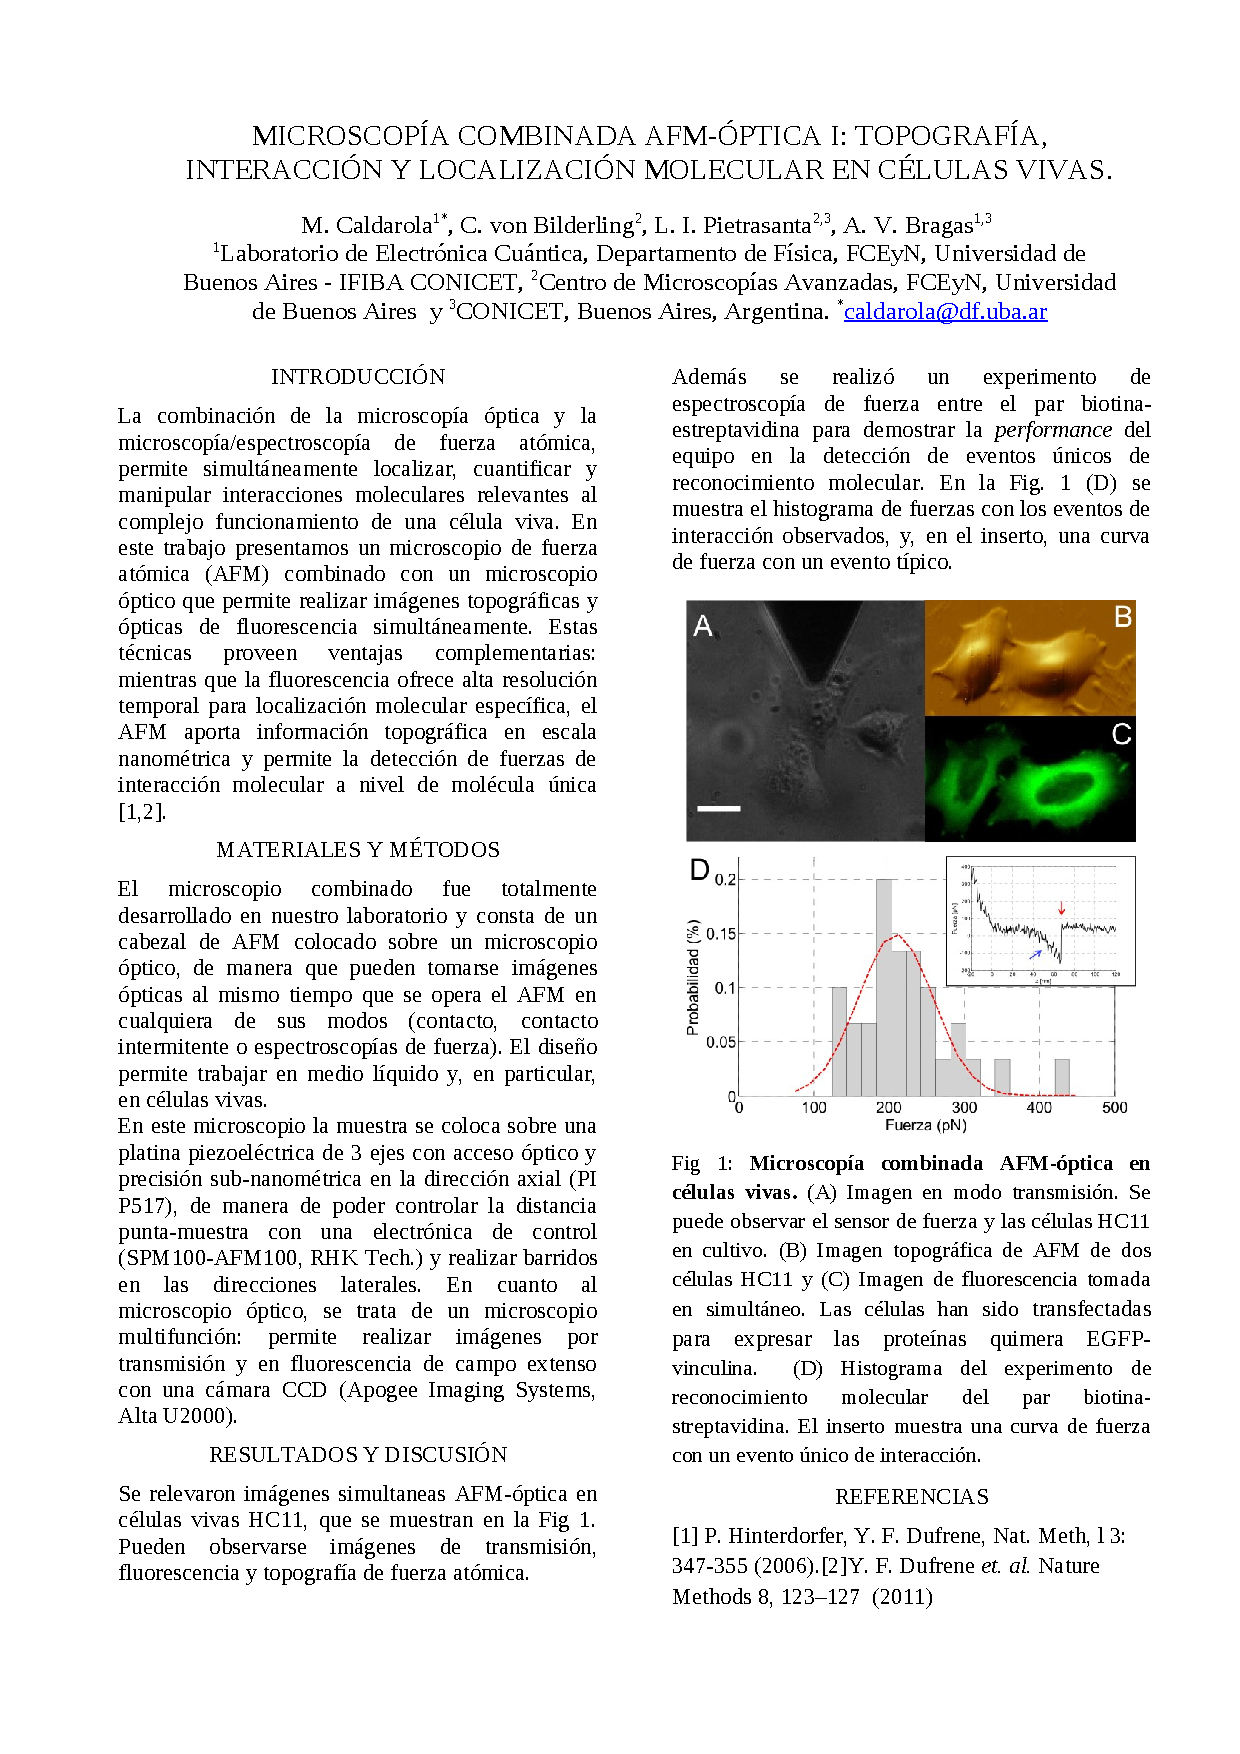
\includepdf[scale=1,addtotoc={1,section,1,{M. Caldarola, C. von Bilderling,
L. I. Pietrasanta y A. V. Bragas, ``\textit{Microscop\'ia combinada
AFM-\'optica: Topograf\'ia, interacci\'on y localizaci\'on en c\'elulas
vivas}''},
MCaldarola},pagecommand=\thispagestyle{plain}]{./abstracts/MCaldarola}

\includepdf[scale=1,addtotoc={1,section,1,{Daneri, Florencia, Gabriel, Manuela y
Aparicio, Rodolfo,
``\textit{An\'alisis t\'ermico por medio de m\'etodos interferom\'etricos}''},
FDaneri },pagecommand=\thispagestyle{plain}]{./abstracts/FDaneri}

\includepdf[scale=1,addtotoc={1,section,1,{Fabricio Della Picca, Ver\'onica
Slezak y Alejandro Peuriot, ``\textit{Caracterizaci\'on de un doblador de
frecuencias \'opticas a partir
de un cristal peri\'odicamente polarizado de LiNbO3 (PPLN)}''},
FDellaPicca},pagecommand=\thispagestyle{plain}]{./abstracts/FDellaPicca}

\includepdf[scale=1,addtotoc={1,section,1,{Guadalupe D\'iaz Costanzo, Laura
Ribba, Silvia Goyanes y Silvia Ledesma, ``\textit{Aumento de la anisotrop\'ia
\'optica en un material polim\'erico fotosensible mediante el agregado de
nanotubos de carbono}''},
GDiazCostanzo},pagecommand=\thispagestyle{plain}]{./abstracts/GDiazCostanzo}

\includepdf[scale=1,addtotoc={1,section,1,{Mar\'ia Celeste Dupla\'a, Leslie
Grant y Ver\'onica V\'azquez, ``\textit{Transmisividad a trav\'es de capas
diel\'ectricas: c\'alculo exacto y
aproximado}''}, CDuplaa},pagecommand=\thispagestyle{plain}]{./abstracts/CDuplaa}

\includepdf[scale=1,addtotoc={1,section,1,{Etcheverry, Mar\'ia Eugenia,
Pasquale, Miguel Angel y Garavaglia, Mario,
``\textit{Evidencias f\'isicas experimentales que justifican resultados
biol\'ogicos en la Terapia Fotodin\'amica del C\'ancer}''},
MEtcheverry},pagecommand=\thispagestyle{plain}]{./abstracts/MEtcheverry}

\includepdf[scale=1,addtotoc={1,section,1,{J. Gargiulo, F. D. Stefani,
``\textit{Impresi\'on de nanopart\'iculas individuales mediante
fuerzas \'opticas}''},
JGargiulo},pagecommand=\thispagestyle{plain}]{./abstracts/JGargiulo}

\includepdf[scale=1,addtotoc={1,section,1,{Rodrigo Mart\'inez Gazoni, Mar\'ia
Luz Mart\'inez Ricci, Martin Bellino, M. Cecilia Fuertes y Galo Soler-Illia,
``\textit{Localizaci\'on espacial y amplificaci\'on de campo en
Cristales Fot\'onicos Mesoporosos con Inclusi\'on de NPs de Ag}''},
RGazoni},pagecommand=\thispagestyle{plain}]{./abstracts/RGazoni}

\includepdf[scale=1,addtotoc={1,section,1,{G. Grinblat, L. J. Borrero
Gonz\'alez, L. A. O. Nunes, M. Tirado, y D. Comedi,
``\textit{Mejoramiento de la emisividad UV en nanohilos de ZnO
por recubrimiento con MgO}''},
GGrinblat},pagecommand=\thispagestyle{plain}]{./abstracts/GGrinblat}

\includepdf[scale=1,addtotoc={1,section,1,{G. Grinblat, M.G. Capeluto,
M. Tirado, D. Comedi, A.V. Bragas, ``\textit{Nanoestructuras de ZnO fabricadas
por transporte de vapor: Correlaci\'on entre par\'ametros de crecimiento y
luminiscencia}''},
GGrinblat2},pagecommand=\thispagestyle{plain}]{./abstracts/GGrinblat2}

\includepdf[scale=1,addtotoc={1,section,1,{M. N. Guzm\'an, L. I. Passoni, H. J.
Rabal, M. Trivi,
``\textit{Speckle en procesos din\'amicos: nuevos aportes}''},
MGuzman},pagecommand=\thispagestyle{plain}]{./abstracts/MGuzman}

\includepdf[scale=1,addtotoc={1,section,1,{Laura Knoll, Christian Schmiegelow
y Miguel Larotonda, ``\textit{Implementaci\'on experimental del algoritmo de
teleportaci\'on cu\'antica}''},
LKnoll},pagecommand=\thispagestyle{plain}]{./abstracts/LKnoll}

\includepdf[scale=1,addtotoc={1,section,1,{Ignacio H. L\'opez Grande, Christian
T. Schmiegelow y Miguel A. Larotonda, ``\textit{Prototipo Aut\'onomo de
Distribuci\'on Cu\'antica de Claves}''},
ILopezGrande},pagecommand=\thispagestyle{plain}]{./abstracts/ILopezGrande}

\includepdf[scale=1,addtotoc={1,section,1,{Marcelo A. Luda , Christian T.
Schmiegelow y Miguel A. Larotonda, ``\textit{Caracterizaci�n de un separador de
modos espaciales de la luz y dise\~no experimental para implementaci\'on de QKD
con 2 qubits}''},
MLuda},pagecommand=\thispagestyle{plain}]{./abstracts/MLuda}

\includepdf[scale=1,addtotoc={1,section,1,{Eduardo D. Mart\'inez, Ver\'onica M.
S\'anchez, Galo J. A. A. Soler-Illia, ``\textit{Caracterizaci\'on y modelado de
propiedades \'opticas de nanopart\'iculas met\'alicas en pel\'iculas delgadas
mesoporosas}''},
EMartinez},pagecommand=\thispagestyle{plain}]{./abstracts/EMartinez}

\includepdf[scale=1,addtotoc={1,section,1,{Leonardo Morbidel, Laureano A. Bulus
Rossini, Pablo A. Costanzo Caso,
``\textit{Antena de banda ancha para sistemas de Radio sobre Fibra \'optica
(RoF)}''},
LMorbidel },pagecommand=\thispagestyle{plain}]{./abstracts/LMorbidel}

\includepdf[scale=1,addtotoc={1,section,1,{Bruno Moretti, Christian T.
Schmiegelow y Miguel A. Larotonda,
``\textit{Medici\'on de estad\'istica de fotones con alta resoluci\'on
temporal}''},
BMoretti},pagecommand=\thispagestyle{plain}]{./abstracts/BMoretti}

\includepdf[scale=1,addtotoc={1,section,1,{Alejandro Natoli, Laureano A. Bulus
Rossini, Pablo A. Costanzo Caso,
``\textit{Plataforma de comunicaciones Gigabit Ethernet \'optica en
FPGA}''},
ANatoli},pagecommand=\thispagestyle{plain}]{./abstracts/ANatoli}

\includepdf[scale=1,addtotoc={1,section,1,{Diego J. A. Ocampo, Cristian L.
Arrieta, Claudio A. Gillari, Lidia T.
Alaniz, Dario David de Lima,
``\textit{Filtro \'optico de multicapa diel\'ectrica}''},
DOcampo},pagecommand=\thispagestyle{plain}]{./abstracts/DOcampo}

\includepdf[scale=1,addtotoc={1,section,1,{Pamela Pardini, O. Di Rocco, D.
Iriarte, J. A. Pomarico y H. F.
Ranea-Sandoval,
``\textit{T\'ecnica fotoac\'ustica en mezclas binarias de
l\'iquidos. Reconstrucci\'on de la se\~nal y propiedades termodin\'amicas en
exceso}''},
PPardini},pagecommand=\thispagestyle{plain}]{./abstracts/PPardini}

\includepdf[scale=1,addtotoc={1,section,1,{Rodrigo A. Ponzio, Mario R. Romero,
Jorge E. Perez y Rodrigo E. Palacios,
``\textit{Dise\~no y fabricaci\'on de un microscopio de fluorescencia para
detecci\'on de mol\'eculas/part\'iculas individuales}''},
RPonzio},pagecommand=\thispagestyle{plain}]{./abstracts/RPonzio}

\includepdf[scale=1,addtotoc={1,section,1,{Heinrich Sebastian Rabal, Laureano A.
Bulus Rossini, Pablo A. Costanzo Caso,
``\textit{Resonador \'optico en anillo y su aplicaci\'on en la
implementaci\'on de l\'ineas de retardo controlables}''},
SRabal},pagecommand=\thispagestyle{plain}]{./abstracts/SRabal}

\includepdf[scale=1,addtotoc={1,section,1,{Leandro Rivero Gonzalez, Ariel
Lutenberg y Natalia \'Alvarez, ``\textit{Caracterizaci\'on de circuitos
integrados de fotodetecci\'on para codificadores \'opticos basados en haces no
difractivos}''},LRivero},pagecommand=\thispagestyle{plain}]{./abstracts/LRivero}

\includepdf[scale=1,addtotoc={1,section,1,{Romano, C. G. C. , Verstraeten, F. ,
Aranda, C. Z. , Burman A. , Skop, G. y Veiras, F.,
``\textit{Controlador electr\'onico para un Espectrofocolor\'imetro,
Proyecto de Desarrollo}''},
CRomano},pagecommand=\thispagestyle{plain}]{./abstracts/CRomano}

\includepdf[scale=1,addtotoc={1,section,1,{Sanchez D. , Gladstein D. , Santiago
G. y Gonzalez M.,
``\textit{Aprendiendo din\'amica del l\'aser con componentes ``no
apareados''}''},
DSanchez},pagecommand=\thispagestyle{plain}]{./abstracts/DSanchez}

\includepdf[scale=1,addtotoc={1,section,1,{J. M. J. Santill\'an , L. B.
Scaffardi, F. A. Videla y D. C. Schinca,
``\textit{Funci\'on diel\'ectrica y espectroscop\'ia de extinci\'on
\'optica para la determinaci\'on del tama\~no de nanopart\'iculas de Ag
generadas por ablaci\'on l\'aser de pulsos ultracortos}''},
JSantillan},pagecommand=\thispagestyle{plain}]{./abstracts/JSantillan}

\includepdf[scale=1,addtotoc={1,section,1,{J. M. J. Santill\'an , F. A. Videla,
D. C. Schinca y L. B. Scaffardi,
``\textit{Espectroscop\'ia de extinci\'on para la determinaci\'on de
estructura, configuraci\'on y tama\~no de nanopart\'iculas de Cu
generadas por ablaci\'on con l\'aser de femtosegundo en l\'iquidos}''},
JSantillan2},pagecommand=\thispagestyle{plain}]{./abstracts/JSantillan2}

\includepdf[scale=1,addtotoc={1,section,1,{D. C. Skigin, M. Lester,
``\textit{Transmisi\'on Extraordinaria en Estructuras Peri\'odicas de
Nanoalmbres con Doble Per\'iodo Bajo Incidencia Evanescente}''},
DSkigin},pagecommand=\thispagestyle{plain}]{./abstracts/DSkigin}

\includepdf[scale=1,addtotoc={1,section,1,{Pedro Soubelet, Axel Bruchhausen y
Alejandro Fainstein,``\textit{Espectroscop\'ia Raman en Superredes
Semiconductoras de AlAs-GaAs}''}, PSoubelet
},pagecommand=\thispagestyle{plain}]{./abstracts/PSoubelet}

\includepdf[scale=1,addtotoc={1,section,1,{Ullua Y., Zalcman A., Alvarez N.,
Ciocci Brazzano L., Acosta E., Santiago G. y
Gonzalez M., ``\textit{Sistema fotoac\'ustico para la detecci\'on de
nanopart\'iculas
de oro: teor\'ia y experimento}''},
YUllua},pagecommand=\thispagestyle{plain}]{./abstracts/YUllua}

\includepdf[scale=1,addtotoc={1,section,1,{Ana Laura Vadnjal, Pablo
Etchepareborda y Alejandro Federico, ``\textit{Medici\'on de micro y
nanodesplazamientos en el plano
usando transformada wavelet de patrones de speckle}''},
AVadnjal},pagecommand=\thispagestyle{plain}]{./abstracts/AVadnjal}

\includepdf[scale=1,addtotoc={1,section,1,{J. Varga, L. Reb\'on, S.
Ledesma y C. Iemmi, ``\textit{Representaci\'on de qudits espaciales en un
modulador de
luz}''},
JVarga},pagecommand=\thispagestyle{plain}]{./abstracts/JVarga}

\includepdf[scale=1,addtotoc={1,section,1,{V. Villafa\~ne,
``\textit{Espectroscop\'ia Raman en Microcavidades \'opticas}''},
VVillafane},pagecommand=\thispagestyle{plain}]{./abstracts/VVillafane}

\includepdf[scale=1,addtotoc={1,section,1,{Mariana A. Zeller, Mauro
Cuevas y Ricardo A. Depine,
``\textit{Polaritones Superficiales Plasm\'onicos en estructuras
multicapas con metamateriales}''},
MZeller},pagecommand=\thispagestyle{plain}]{./abstracts/MZeller}